\chapter*{ Anexo II} 

Se presentan una serie de gr\'aficos correspondientes a la distribuci\'on de la fuerza promedio con respecto al tiempo, se obtienen valores para la fuerza promedio de las part\'iculas finas y gruesas cada 50 iteraciones. La informaci\'on corresponde a los modelos uniformemente distribuidos. Esta informaci\'on se utiliza para la confecci\'on de la Figura \ref{fig:GvsR}. \\ 

\begin{figure}[H]
\centering
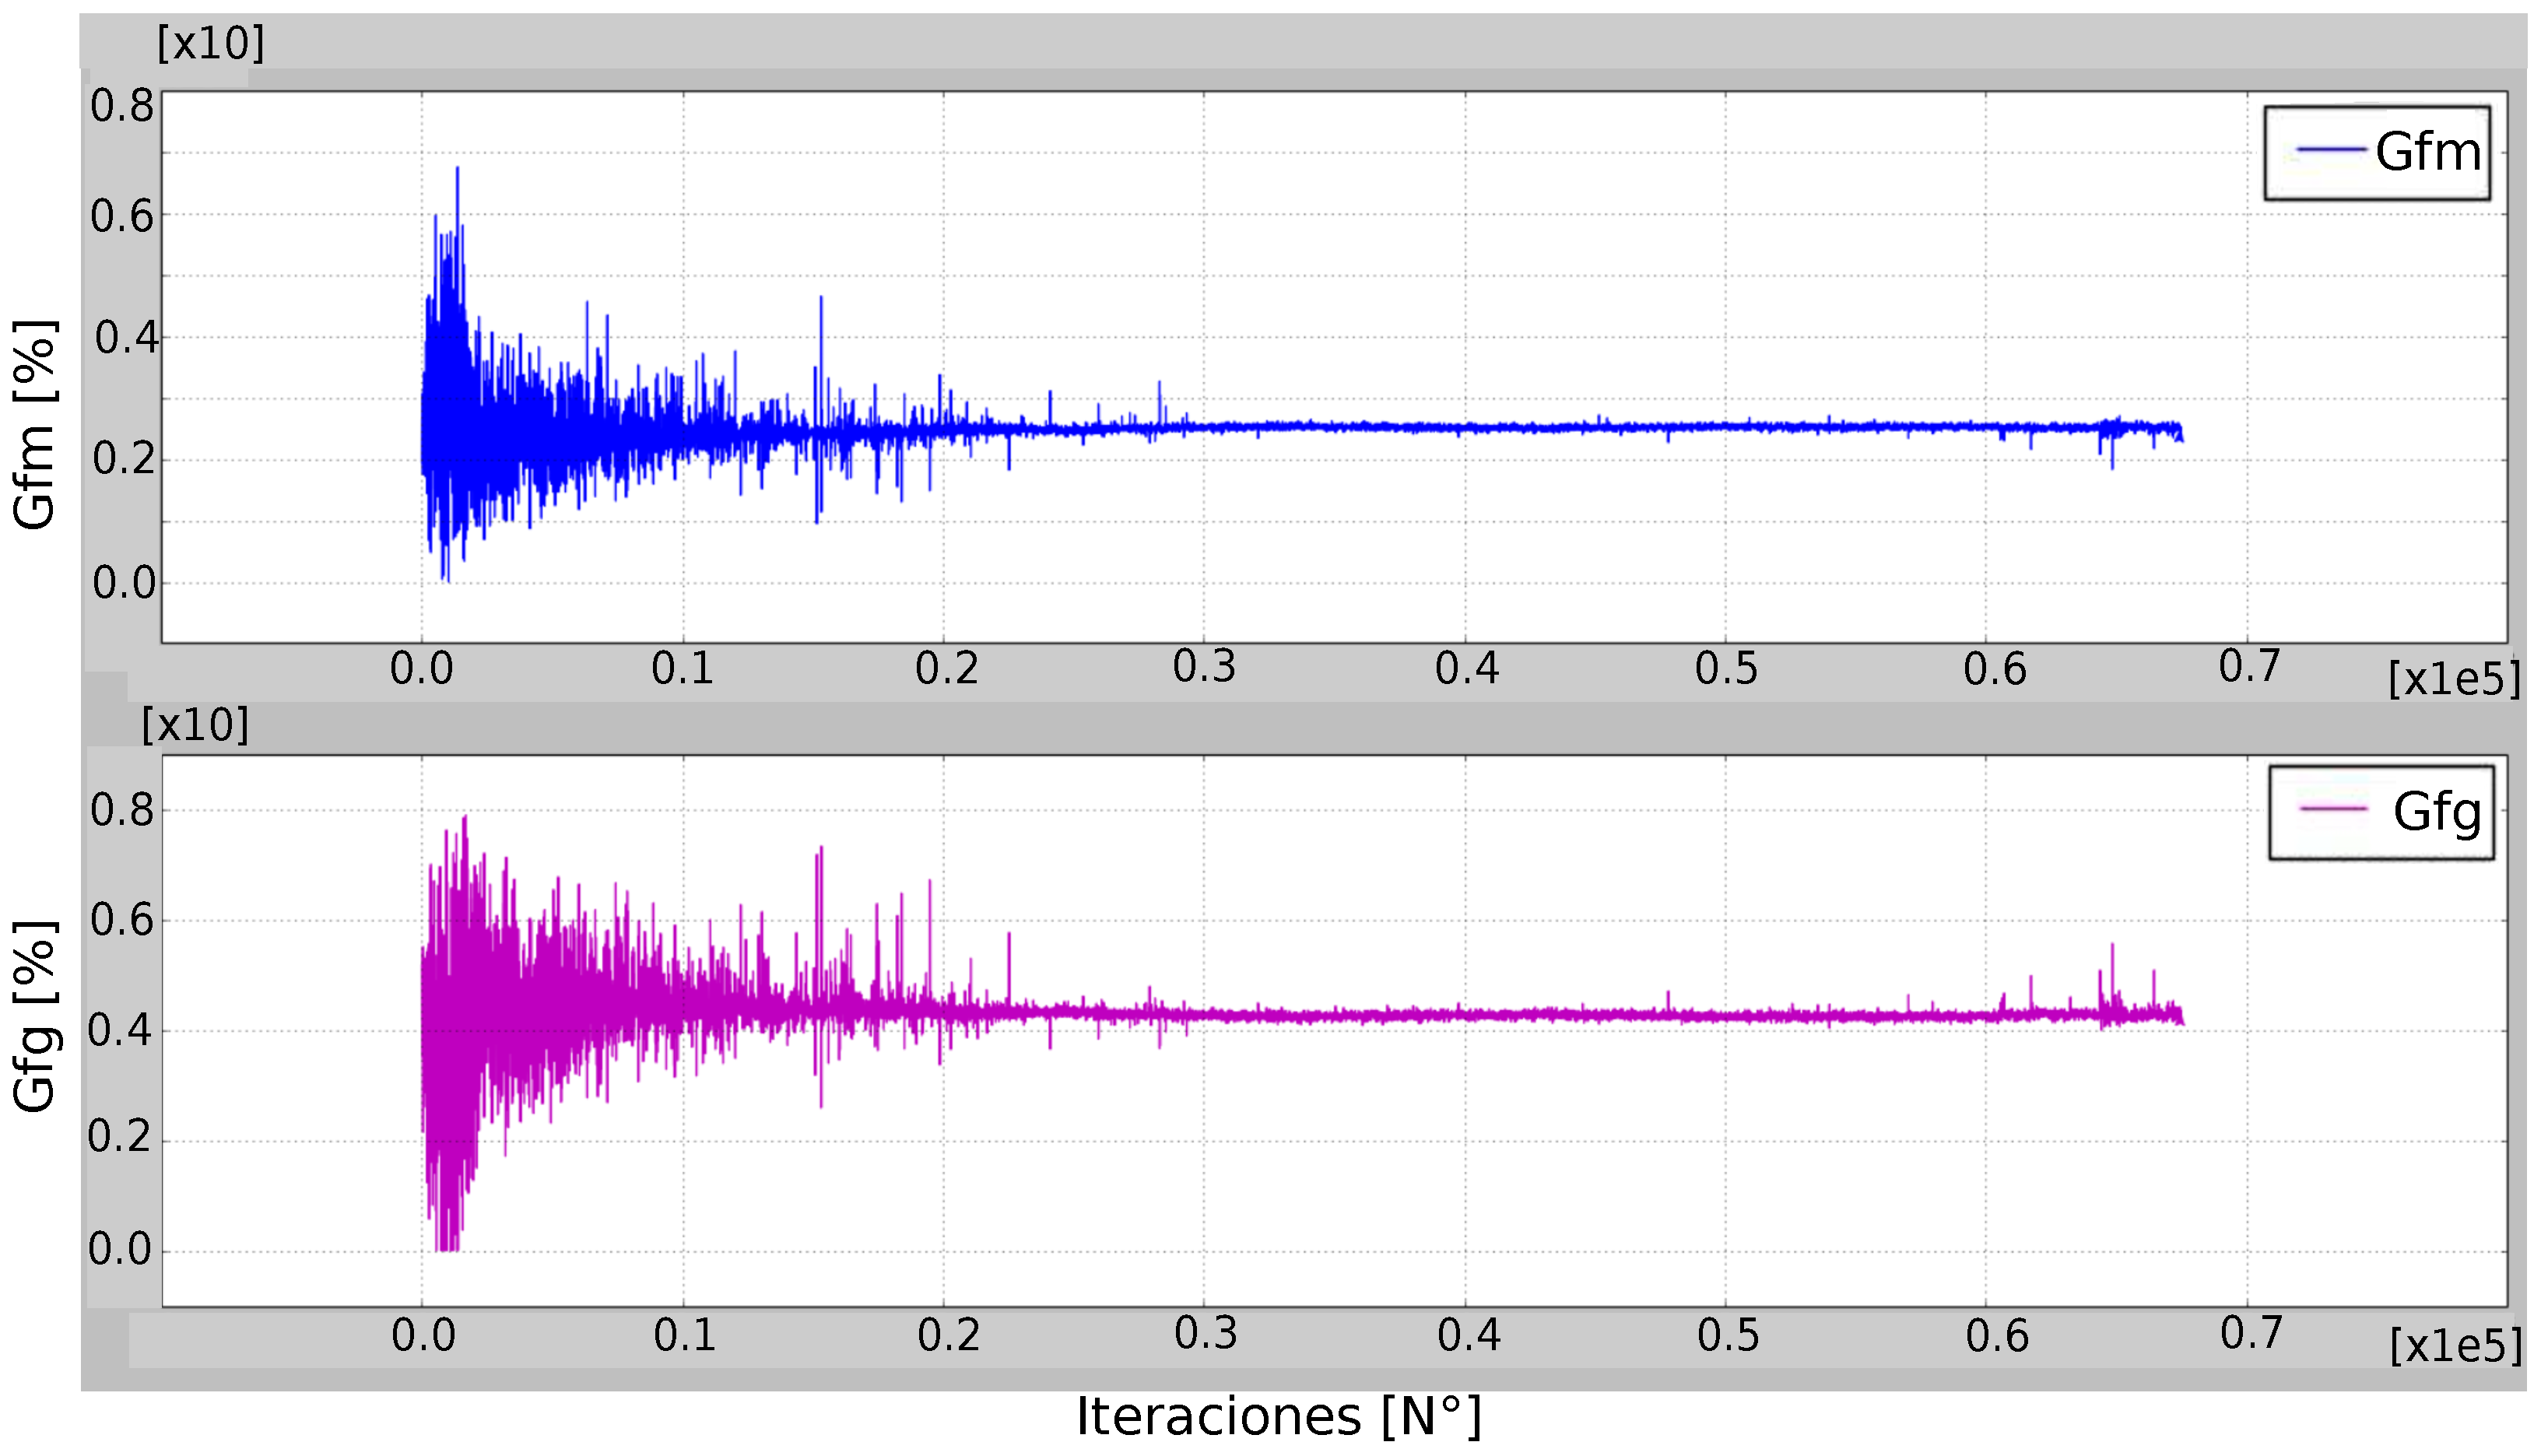
\includegraphics[width=\textwidth]{Anexo1/PSD17}
\caption{Distribuci\'on de fuerzas promedio de granos finos y gruesos para Sd=0.17.}
\label{fig:PSD17}
\end{figure}\\


\begin{figure}[H]
\centering
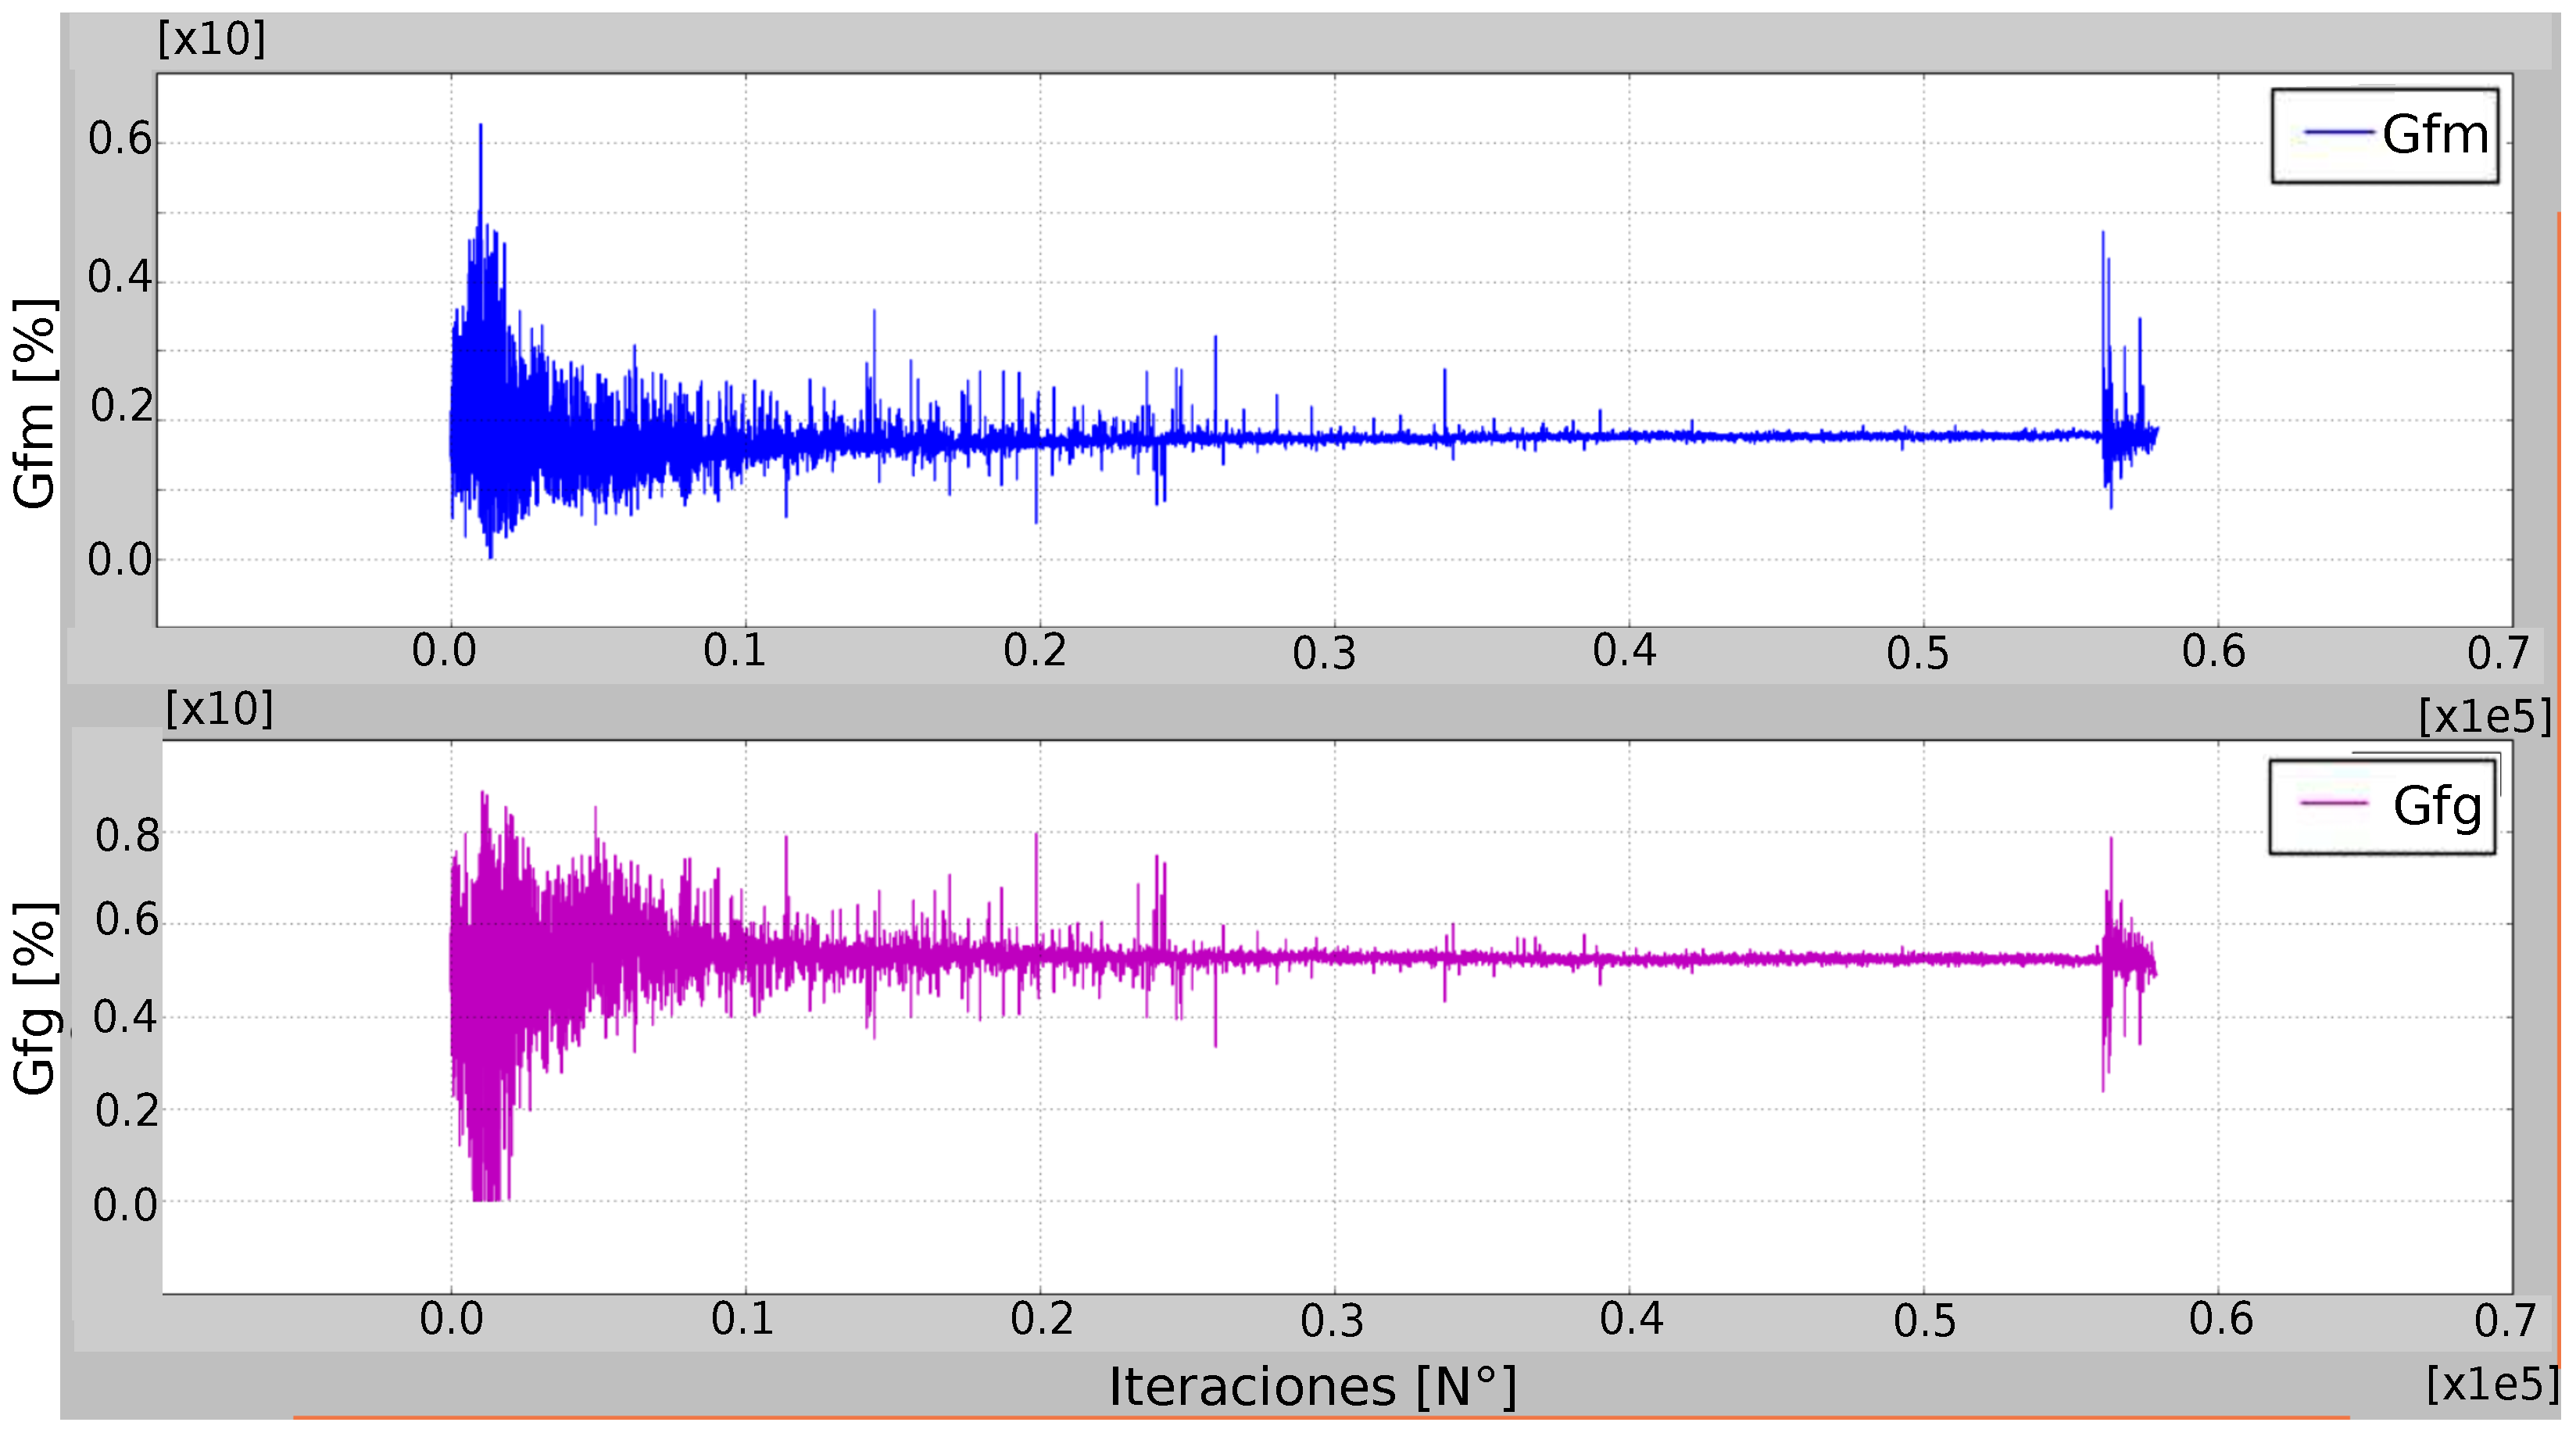
\includegraphics[width=\textwidth]{Anexo1/PSD34}
\caption{Distribuci\'on de fuerzas promedio de granos finos y gruesos para Sd=0.34.}
\label{fig:PSD34}
\end{figure}\\


\begin{figure}[htb]
\centering
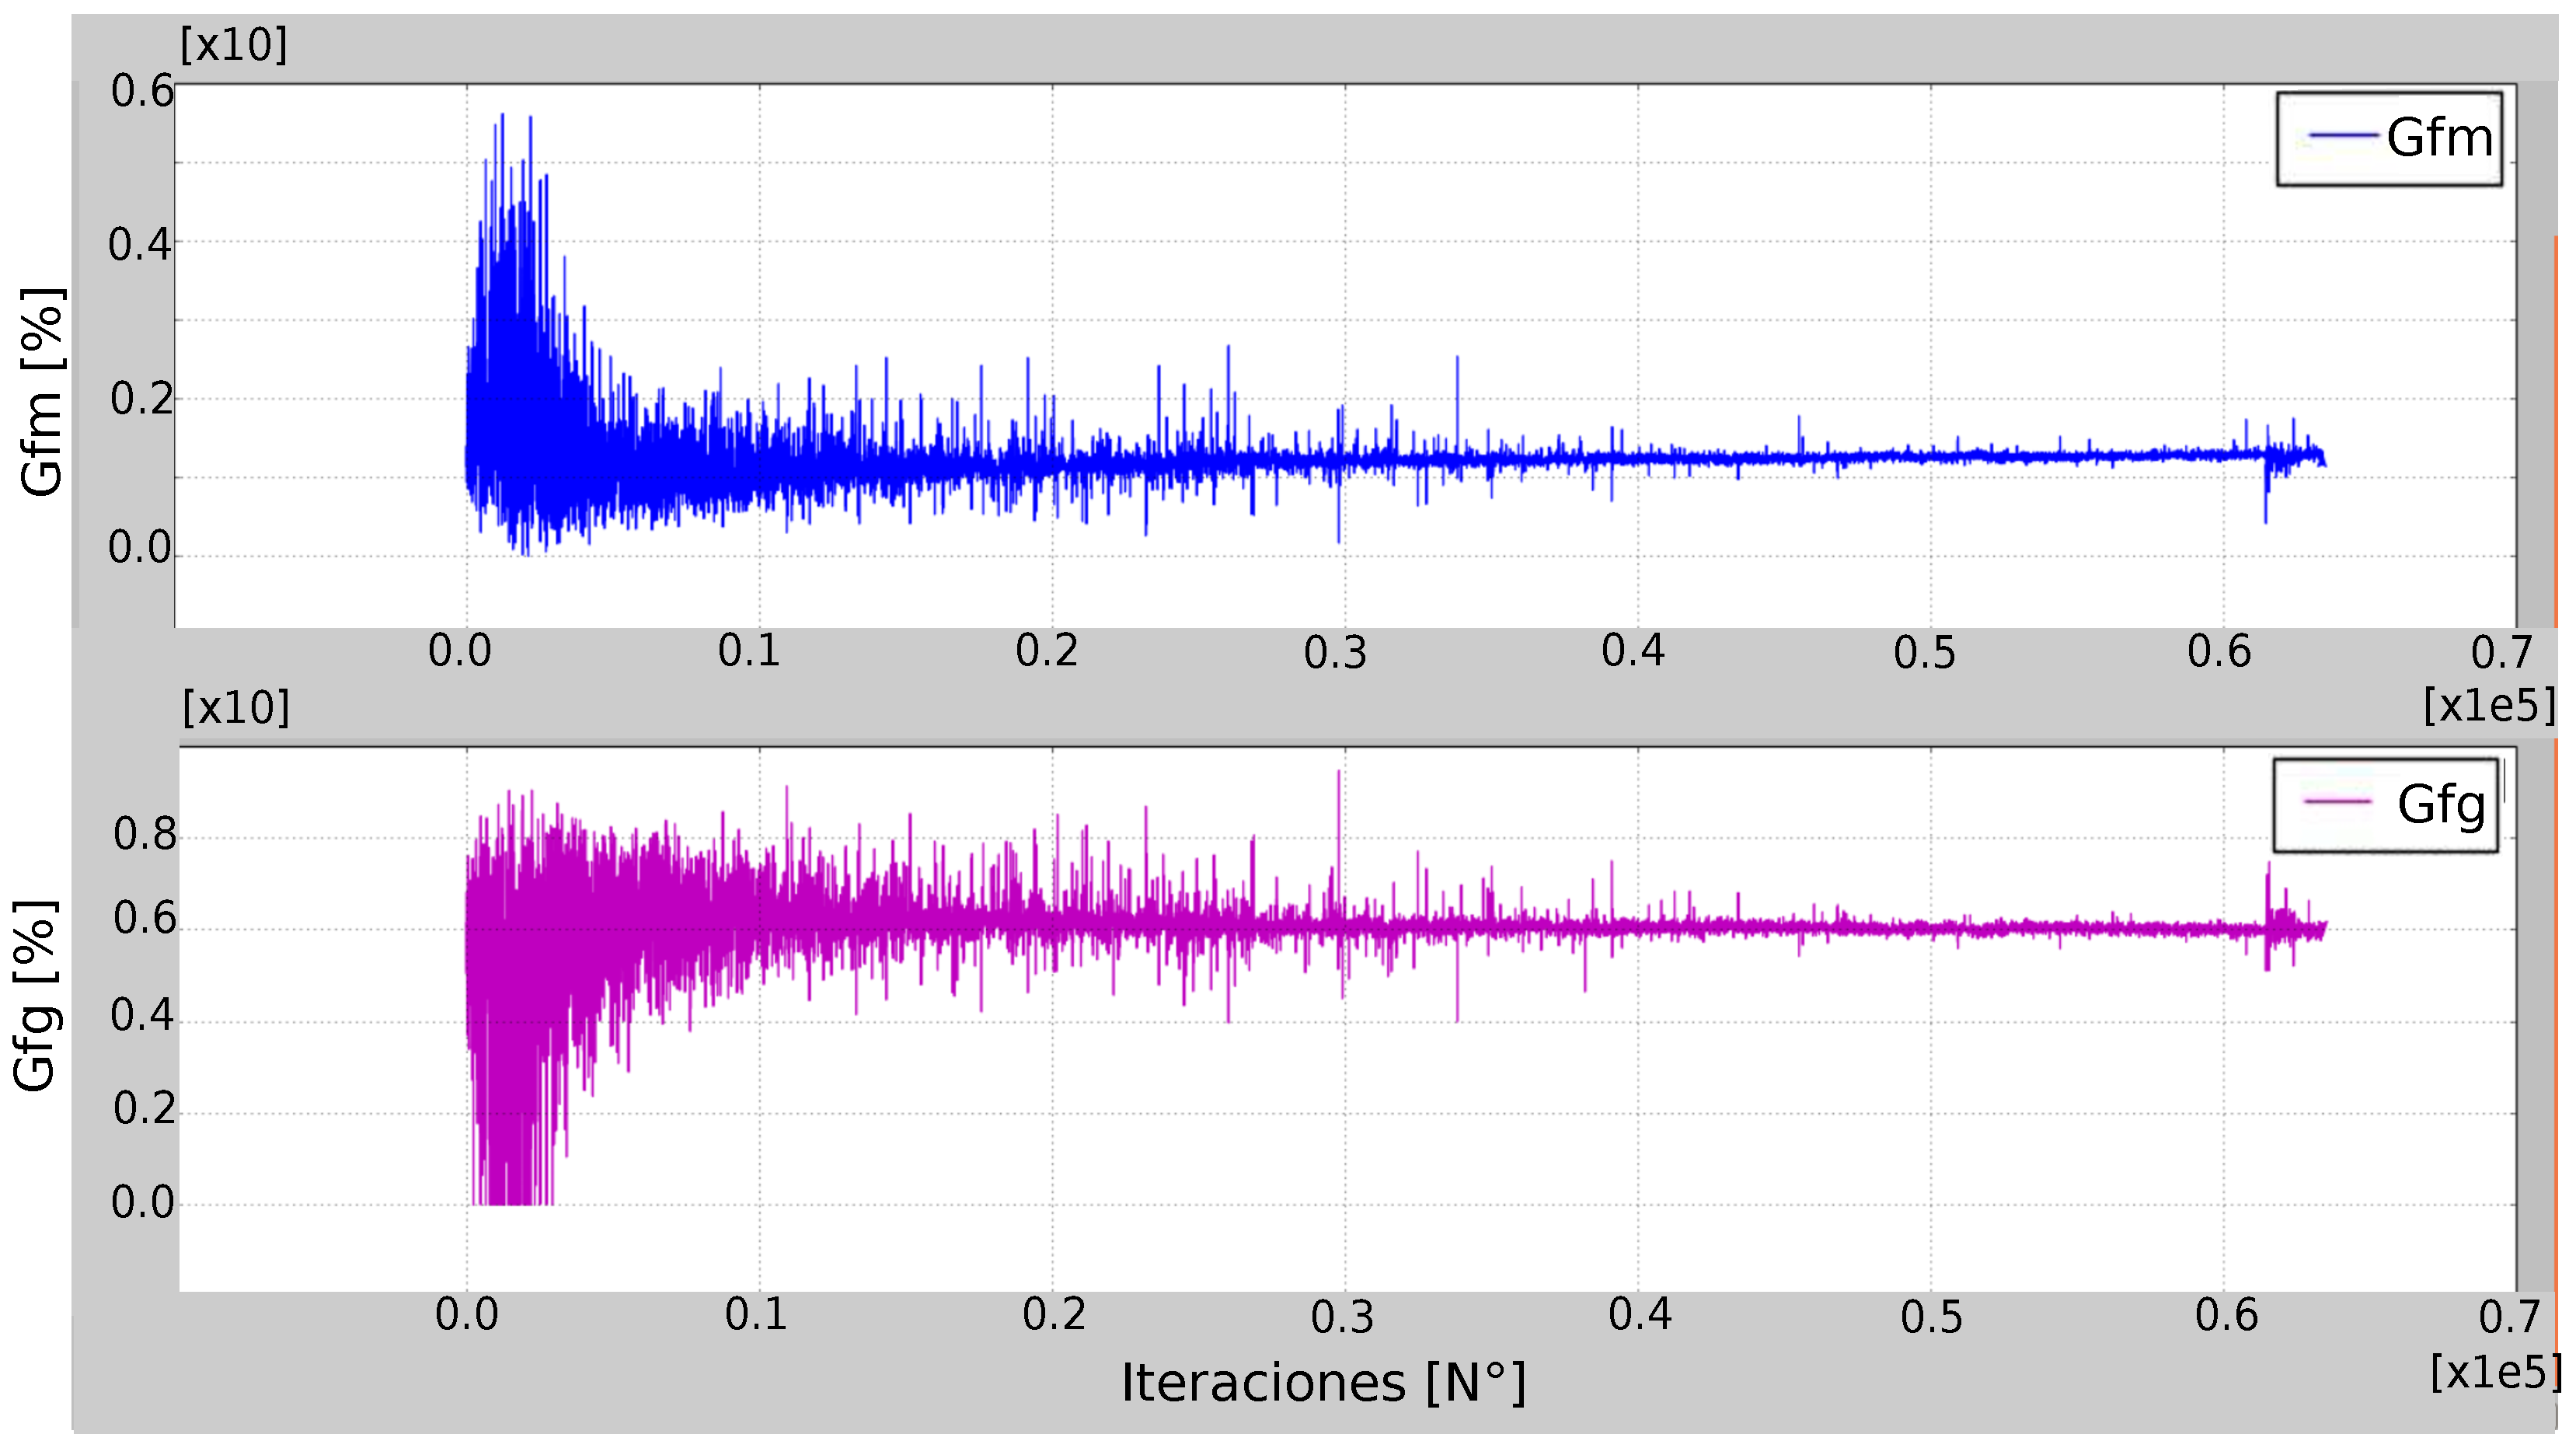
\includegraphics[width=\textwidth]{Anexo1/PSD51}
\caption{Distribuci\'on de fuerzas promedio de granos finos y gruesos para Sd=0.51.}
\label{fig:PSD51}
\end{figure}

\begin{figure}[htb]
\centering
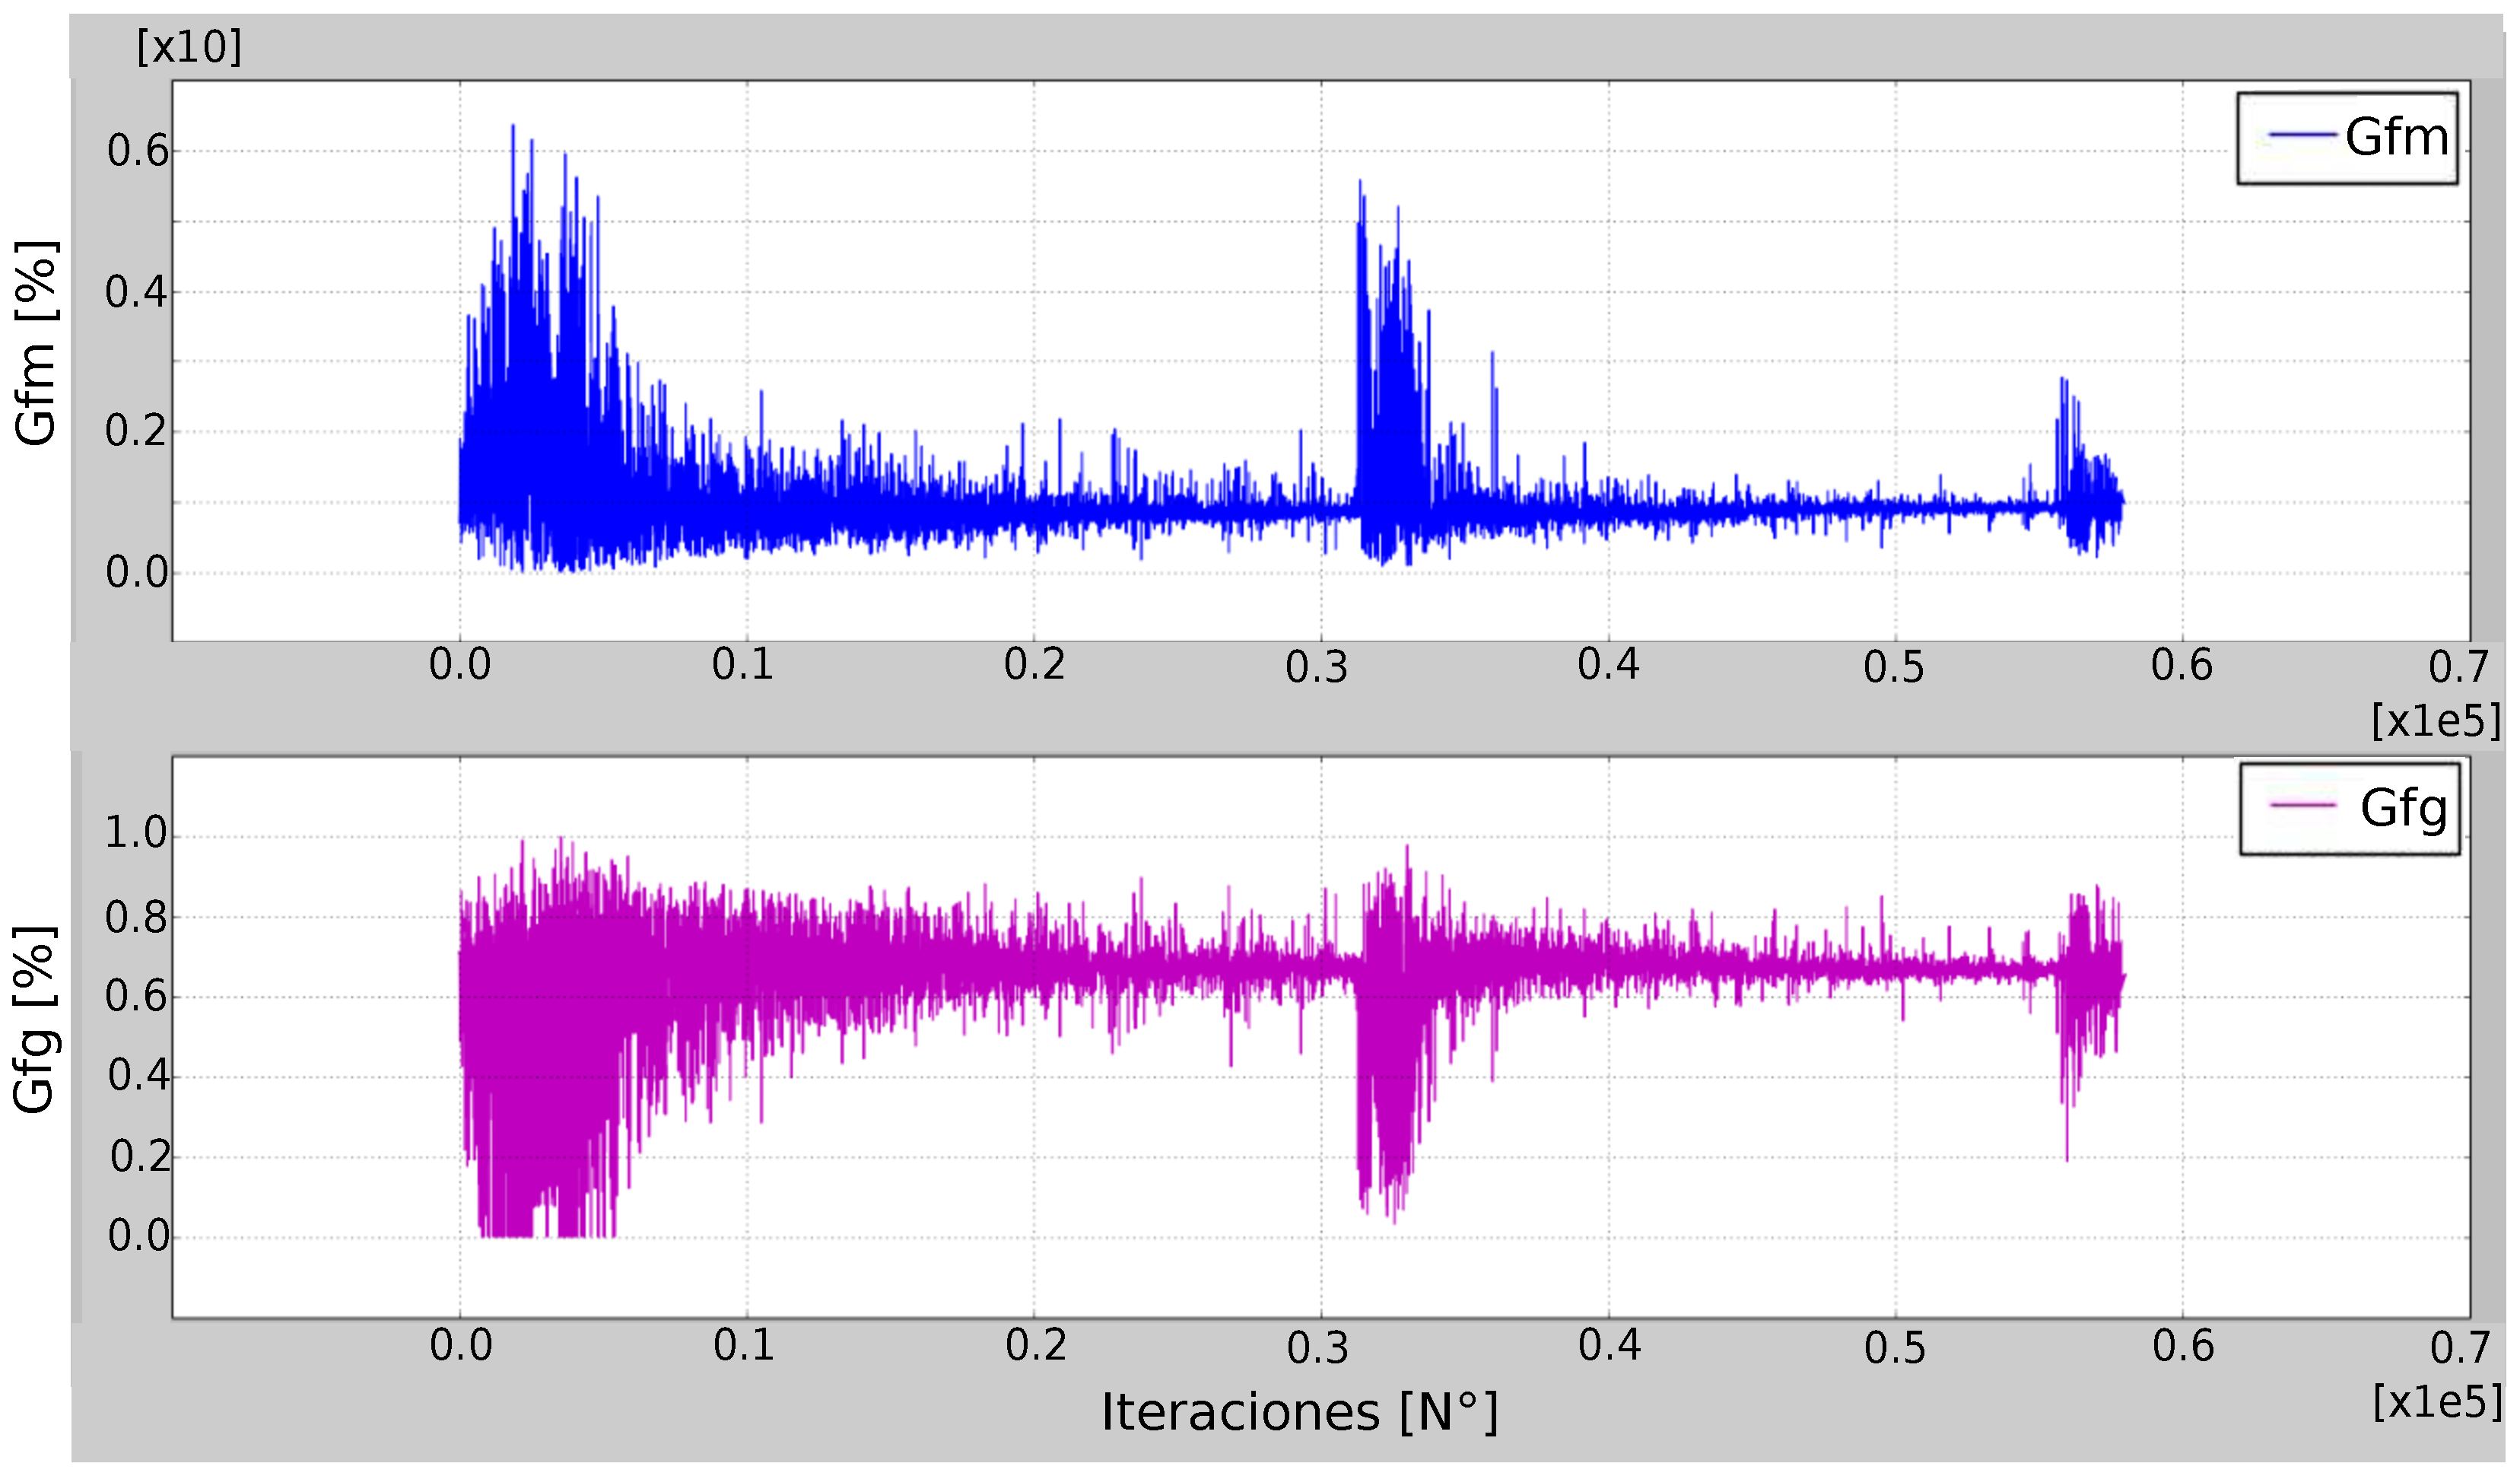
\includegraphics[width=\textwidth]{Anexo1/PSD68}
\caption{Distribuci\'on de fuerzas promedio de granos finos y gruesos para Sd=0.68.}
\label{fig:PSD68}
\end{figure}


\begin{figure}[htb]
\centering
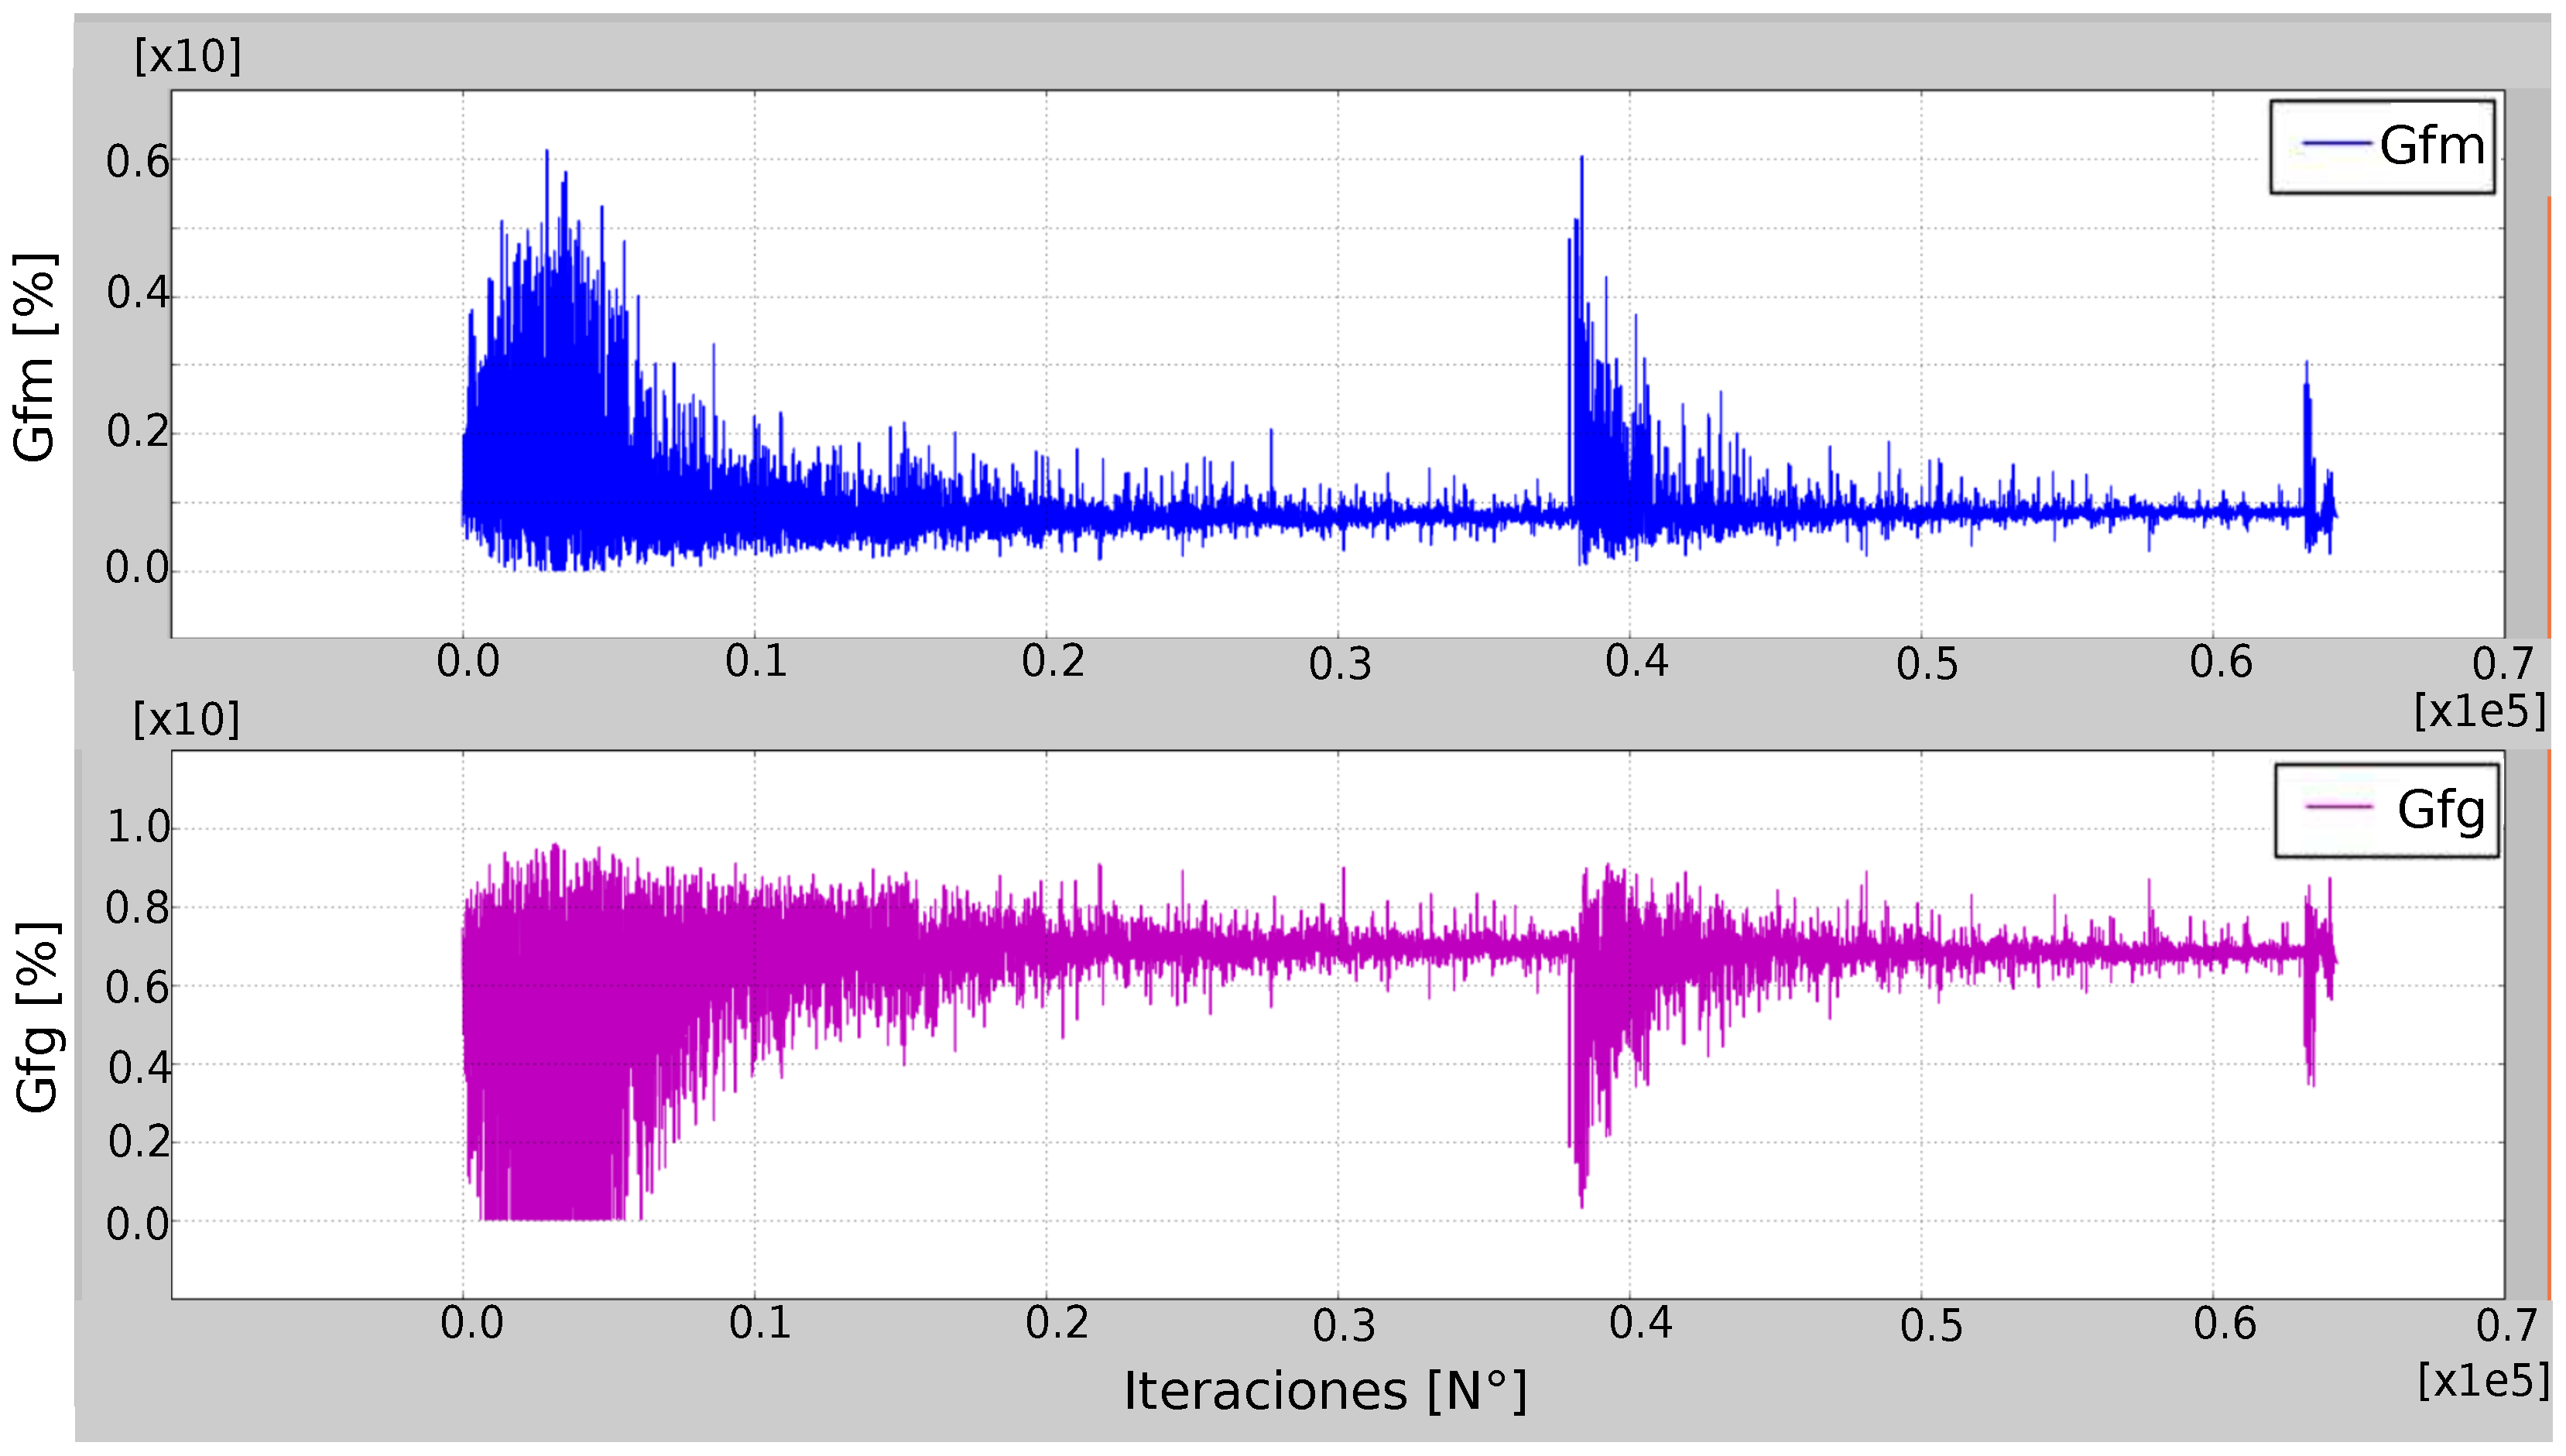
\includegraphics[width=\textwidth]{Anexo1/PSD75}
\caption{Distribuci\'on de fuerzas promedio de granos finos y gruesos para Sd=0.75.}
\label{fig:PSD75}
\end{figure}









